\documentclass[11pt,a4paper]{article}

% Packages
\usepackage[utf8]{inputenc}
\usepackage[margin=1in]{geometry}
\usepackage{graphicx}
\usepackage{hyperref}
\usepackage{xcolor}
\usepackage{fancyhdr}
\usepackage{titlesec}
\usepackage{tocloft}
\usepackage{listings}
\usepackage{enumitem}
\usepackage{booktabs}
\usepackage{tikz}
\usetikzlibrary{shapes,arrows,positioning}

% Color definitions
\definecolor{primarycolor}{RGB}{0,102,204}
\definecolor{secondarycolor}{RGB}{102,102,102}
\definecolor{codebackground}{RGB}{245,245,245}

% Hyperlink setup
\hypersetup{
    colorlinks=true,
    linkcolor=primarycolor,
    filecolor=primarycolor,
    urlcolor=primarycolor,
    citecolor=primarycolor,
    pdftitle={High-Level Design Document},
    pdfauthor={Author Name}
}

% Section formatting
\titleformat{\section}
{\color{primarycolor}\normalfont\Large\bfseries}
{\thesection}{1em}{}

\titleformat{\subsection}
{\color{secondarycolor}\normalfont\large\bfseries}
{\thesubsection}{1em}{}

% Header and footer
\pagestyle{fancy}
\fancyhf{}
\fancyhead[L]{\leftmark}
\fancyhead[R]{\thepage}
\fancyfoot[C]{\scriptsize High-Level Design Document}
\renewcommand{\headrulewidth}{0.5pt}
\renewcommand{\footrulewidth}{0.5pt}

% Code listing style
\lstset{
    backgroundcolor=\color{codebackground},
    basicstyle=\ttfamily\small,
    breaklines=true,
    captionpos=b,
    frame=single,
    numbers=left,
    numberstyle=\tiny\color{secondarycolor},
    keywordstyle=\color{primarycolor}\bfseries,
    commentstyle=\color{secondarycolor}\itshape,
    stringstyle=\color{red!60!black}
}

% Document information
\title{\textbf{\Huge High-Level Design Document}\\[0.5em]
\Large System/Project Name}
\author{Author Name \\ Organization/Team}
\date{\today \\ Version 1.0}

\begin{document}

% Title page
\maketitle
\thispagestyle{empty}

\vspace{2cm}

\begin{center}
\begin{tabular}{|l|l|}
\hline
\textbf{Document Version} & 1.0 \\ \hline
\textbf{Last Updated} & \today \\ \hline
\textbf{Status} & Draft / Review / Approved \\ \hline
\textbf{Owner} & Author Name \\ \hline
\textbf{Reviewers} & Reviewer 1, Reviewer 2 \\ \hline
\end{tabular}
\end{center}

\newpage

% Revision history
\section*{Revision History}
\begin{center}
\begin{tabular}{|c|c|p{6cm}|l|}
\hline
\textbf{Version} & \textbf{Date} & \textbf{Description} & \textbf{Author} \\ \hline
1.0 & \today & Initial draft & Author Name \\ \hline
 &  &  &  \\ \hline
 &  &  &  \\ \hline
\end{tabular}
\end{center}

\newpage

% Table of contents
\tableofcontents
\newpage

% Main content begins
\section{Executive Summary}
Provide a brief overview of the system, its purpose, and key design decisions. This section should be readable by non-technical stakeholders.

\subsection{Purpose}
Describe the purpose of this document and the system it describes.

\subsection{Scope}
Define what is included and excluded from this design.

\subsection{Key Points}
\begin{itemize}
    \item Key design decision 1
    \item Key design decision 2
    \item Key design decision 3
\end{itemize}

\section{System Overview}

\subsection{Background}
Provide context about why this system is being built and what problem it solves.

\subsection{Goals and Objectives}
\begin{itemize}
    \item Primary goal 1
    \item Primary goal 2
    \item Primary goal 3
\end{itemize}

\subsection{Assumptions and Constraints}
\begin{itemize}
    \item \textbf{Assumptions:} List key assumptions made during design
    \item \textbf{Constraints:} List technical, business, or regulatory constraints
\end{itemize}

\section{Architecture Overview}

\subsection{Architectural Pattern}
Describe the overall architectural pattern (e.g., microservices, layered, event-driven).

% Example architecture diagram using TikZ
\begin{figure}[h]
\centering
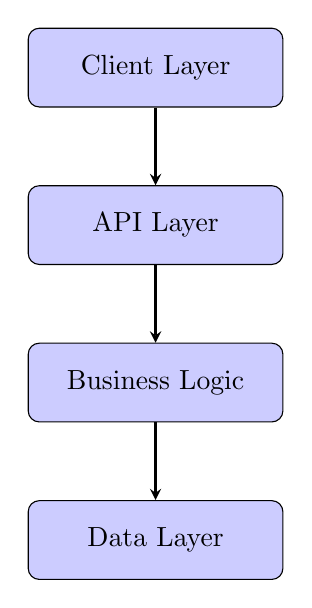
\begin{tikzpicture}[
    node distance=2cm,
    box/.style={rectangle, draw, fill=blue!20, text width=3cm, text centered, rounded corners, minimum height=1cm},
    arrow/.style={->,>=stealth,thick}
]
    \node[box] (client) {Client Layer};
    \node[box, below of=client] (api) {API Layer};
    \node[box, below of=api] (business) {Business Logic};
    \node[box, below of=business] (data) {Data Layer};
    
    \draw[arrow] (client) -- (api);
    \draw[arrow] (api) -- (business);
    \draw[arrow] (business) -- (data);
\end{tikzpicture}
\caption{High-Level Architecture}
\label{fig:architecture}
\end{figure}

\subsection{Key Components}
Describe the major components of the system and their responsibilities.

\section{Component Design}

\subsection{Component 1: [Name]}
\begin{itemize}
    \item \textbf{Purpose:} What this component does
    \item \textbf{Responsibilities:} Key responsibilities
    \item \textbf{Interfaces:} How other components interact with it
    \item \textbf{Dependencies:} What this component depends on
\end{itemize}

\subsection{Component 2: [Name]}
\begin{itemize}
    \item \textbf{Purpose:} What this component does
    \item \textbf{Responsibilities:} Key responsibilities
    \item \textbf{Interfaces:} How other components interact with it
    \item \textbf{Dependencies:} What this component depends on
\end{itemize}

\section{Data Design}

\subsection{Data Models}
Describe key data entities and their relationships.

\subsection{Data Flow}
Explain how data moves through the system.

\subsection{Storage Strategy}
Describe database choices, caching strategies, etc.

\section{Interface Design}

\subsection{API Specifications}
Document key APIs and their contracts.

\begin{lstlisting}[language=json, caption=Example API Request]
{
    "endpoint": "/api/v1/resource",
    "method": "POST",
    "body": {
        "field1": "value1",
        "field2": "value2"
    }
}
\end{lstlisting}

\subsection{External Integrations}
List and describe integrations with external systems.

\section{Security Design}

\subsection{Authentication \& Authorization}
Describe how users are authenticated and authorized.

\subsection{Data Security}
Explain encryption, data protection measures.

\subsection{Security Considerations}
List key security considerations and mitigation strategies.

\section{Performance \& Scalability}

\subsection{Performance Requirements}
Define performance targets (latency, throughput, etc.).

\subsection{Scalability Strategy}
Explain how the system scales (horizontal/vertical, auto-scaling, etc.).

\subsection{Caching Strategy}
Describe caching layers and policies.

\section{Reliability \& Availability}

\subsection{High Availability Design}
Explain redundancy, failover mechanisms.

\subsection{Disaster Recovery}
Describe backup and recovery procedures.

\subsection{Monitoring \& Alerting}
List key metrics to monitor and alerting strategies.

\section{Deployment Architecture}

\subsection{Deployment Model}
Describe cloud provider, containerization, orchestration.

\subsection{Environment Strategy}
Explain dev, staging, production environments.

\subsection{CI/CD Pipeline}
Describe continuous integration and deployment approach.

\section{Technology Stack}

\begin{center}
\begin{tabular}{|l|l|}
\hline
\textbf{Layer} & \textbf{Technology} \\ \hline
Frontend & React, TypeScript \\ \hline
Backend & Node.js, Express \\ \hline
Database & PostgreSQL \\ \hline
Cache & Redis \\ \hline
Message Queue & RabbitMQ \\ \hline
Infrastructure & AWS, Docker, Kubernetes \\ \hline
\end{tabular}
\end{center}

\section{Risks and Mitigation}

\begin{center}
\begin{tabular}{|p{4cm}|p{3cm}|p{5cm}|}
\hline
\textbf{Risk} & \textbf{Impact} & \textbf{Mitigation Strategy} \\ \hline
Technical complexity & High & Phased implementation, prototyping \\ \hline
Third-party dependencies & Medium & Vendor evaluation, fallback options \\ \hline
 &  &  \\ \hline
\end{tabular}
\end{center}

\section{Future Considerations}

\subsection{Known Limitations}
List current limitations of the design.

\subsection{Future Enhancements}
Describe potential future improvements or features.

\section{Appendices}

\subsection{Appendix A: Glossary}
\begin{itemize}
    \item \textbf{Term 1:} Definition
    \item \textbf{Term 2:} Definition
\end{itemize}

\subsection{Appendix B: References}
\begin{itemize}
    \item Reference 1
    \item Reference 2
\end{itemize}

\end{document}